\label{sec:2_related_work}
\section{Related Work} 

In this section, some relevant work for this thesis will be presented. Knowing the main takeaways from these works will help understand the context and assessments that will be made when implementing the methods presented in the next chapter. 
The topics covered in this chapter are computer vision, different methods to create explainable machine learning models, and the development of large language models that lead to the model used in this work.

% Computer vision
% ------------------------------------------
\subsection{Computer Vision}
Computer Vision is the interdisciplinary task of making computers understand and act on visual input. This scientific discipline's main objective is to make computers extract high-dimensional data from the real world using digital images and videos. The extraction of visual information that computers can use includes methods for collecting, processing, analyzing, and understanding the images using statistics, geometry, physics, and learning theory. 

% Object detection
Object detection is a significant part of computer vision that has made astonishing progress. It has been an important research topic because it is one of the fundamental problems in computer vision. Detecting objects form the fundamental basis of other computer vision tasks, such as object tracking, segmentation, and image captioning. Many of these sub-domains' achievements have come from using \gls{cnn} architectures with more layers, trained on larger datasets, and more powerful computers. These main components have made the algorithms capable of learning a deeper understanding of the visual world and learning more fundamental elements of materials, objects, and scenes.  

% Is this relevant?
Krizhevsky et al. introduced AlexNet\cite{krizhevskyImageNetClassificationDeep2017}, as a variant of the \gls{cnn} proposed by LeCun et al.\cite{lecunHandwrittenDigitRecognition1989, lecunGradientbasedLearningApplied1998} seen in Figure \ref{fig:lenet}, both utilizing the backpropagation algorithm \cite{rumelhartLearningRepresentationsBackpropagating1986}
in training. The main difference is that AlexNet uses three more layers, \gls{relu} \cite{fukushimaCognitronSelforganizingMultilayered1975}
, and is running on \glspl{gpu} instead of \glspl{cpu}, which in practice means more efficient use of computing power.
AlexNet achieved impressive results in the ImageNet \cite{dengImageNetLargeScaleHierarchical2009} 2012 Challenge and is often considered the most influential paper published in computer vision. 
Following this paper, there has been an increasing amount of work done and articles published in the domain of deep learning and images during the last decade.

\begin{figure}[htb]
    \centerline{
    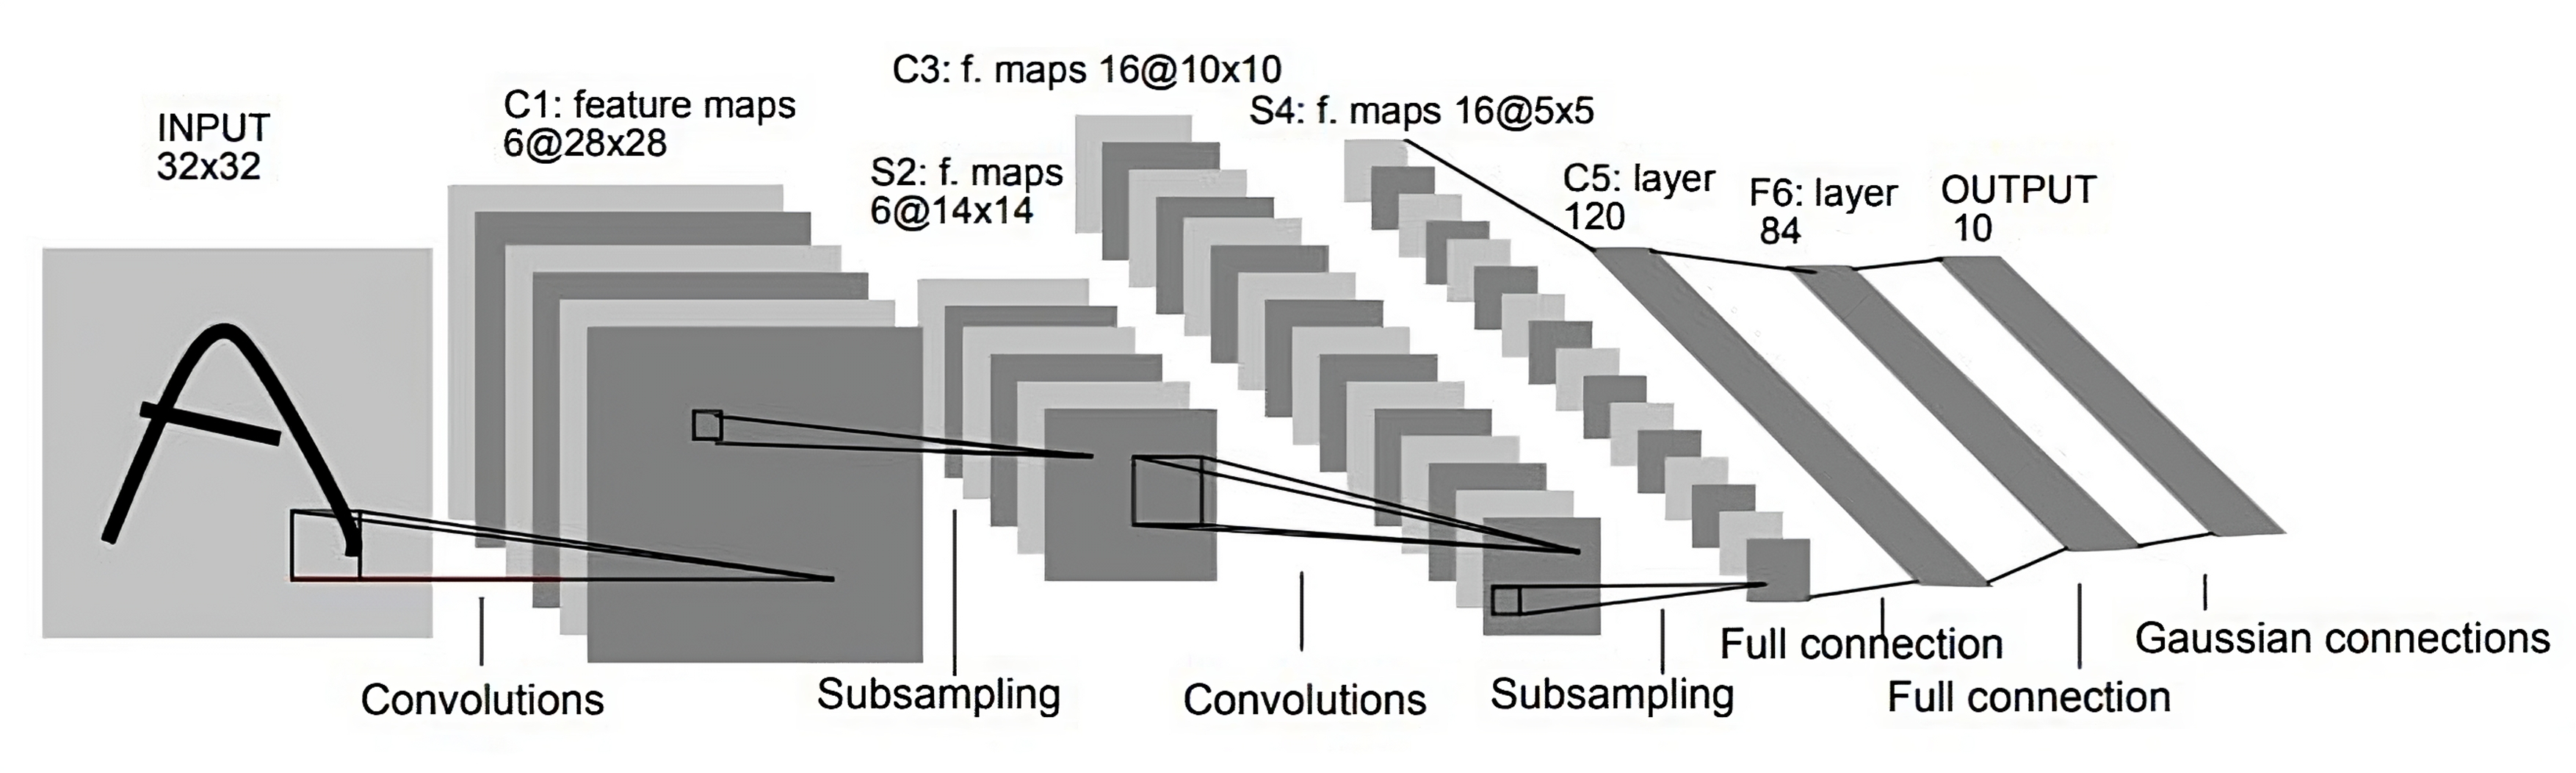
\includegraphics[width=1.2\linewidth]{images/LeNet.jpeg}}
    \caption{\gls{cnn} architecture of LeNet-5 proposed by LeCun et al. \cite{lecunGradientbasedLearningApplied1998}.}
    \label{fig:lenet}
\end{figure} 

% XAI
% ------------------------------------------
\subsection{Explainable AI (XAI)}

The rapid growth of artificial intelligence (AI) technologies has led to an increasing demand for transparency and interpretability in machine learning models. While these models have demonstrated impressive performance in various applications, their lack of transparency and interpretability has raised concerns about their reliability, accountability, and potential biases. As a result, the field of explainable AI (XAI) has emerged to address these challenges by developing techniques and tools that enable humans to understand how AI systems work and make decisions.

Explainable AI is an interdisciplinary research field that aims to make AI models more transparent, interpretable, and accountable to human users. It combines techniques from machine learning, human-computer interaction, cognitive science, and other related disciplines to develop methods and tools for explaining the behavior and decisions of AI models. The need for XAI arises from the fact that many machine learning models, especially deep neural networks, are often viewed as black boxes, meaning that their internal workings and decision-making processes are intricate for humans to comprehend. As a result, these models' lack of transparency and interpretability can create distrust among users, limit their adoption, and raise ethical concerns, especially in high-stakes applications such as healthcare, finance, and criminal justice.

An overview of influential methods proposed in \gls{xai} is presented in this subsection.

% LIME
\paragraph{LIME\\}
In pursuing a method that helps the explaining model to be locally faithful to the underlying model, Ribeiro et al. \cite{ribeiroWhyShouldTrust2016} proposed \gls{lime}. This model-agnostic method explains any method by learning an interpretable, less complex model locally around a specific prediction. This approach assures that the explanation is locally accurate and represents the actual inner workings of the model. 
In the same paper, they also introduce a method for explaining the global attributes of the model by framing the task as a submodular optimization problem. The technique is called SP-LIME (Submodular Pick LIME). With this approach, they can achieve global explanations that are locally accurate and faithful to the underlying model in a non-redundant way. LIME will be used later in this thesis as an explanation method adapted to a \gls{llm}.

% SHAP
\paragraph{SHAP\\}
Making non-redundant explanation features faithfully and efficiently is not easy. Lundberg et al. \cite{lundbergUnifiedApproachInterpreting2017} proposed a unified framework for interpreting predictions made by the underlying method. This framework called \gls{shap}, assigns each feature a value of importance for a specific prediction. The framework utilizes the class of additive feature attribution methods and estimates the Shapley % cite
values from cooperative game theory for that prediction. With this approach, they achieve more effective explanations to compute and have better consistency with human intuition than previously proposed methods.  


% Grad-CAM
\paragraph{Grad-CAM\\}
Visually explaining features that contributed to an image prediction can be essential in gaining trust in a model. Selvaraju et al. \cite{selvarajuGradCAMVisualExplanations2020} proposed a technique for making \glspl{cnn} more explainable and transparent by producing visual explanations for the underlying model. The method is called \gls{gradcam}, a generalization of CAM proposed by Zhou et al. \cite{zhouLearningDeepFeatures2016}, and uses the gradients in a single backtrack of any target concept. Therefore it does not need any architectural changes or retraining of the underlying prediction model to produce a localization map highlighting the crucial regions in the image for predicting the given concept, often called a saliency map in computer vision.

% DenseCap


% FLEX
\paragraph{FLEX\\}
While visual-only explanations can give the user insight into which areas of the image were essential in making the decision, they tell little to nothing about why those regions were important. On the other hand, linguistic descriptions give the user an essential understanding of the model's evaluation when predicting. 
Wickramanayake et al. \cite{wickramanayakeFLEXFaithfulLinguistic2019} propose \gls{flex} to merge saliency maps with locally accurate linguistic descriptions. In this approach, they look at the gradients through layers and identify the most critical activations in the single decision. The advantage of looking at different layers is that alongside getting an explanation that is faithful to the underlying model, they also extract features the \gls{cnn} identifies at each layer. A \gls{cnn} may represent high-level concepts, like a "car", at the last layer while identifying features such as texture and color at earlier layers. Using the activations at all essential layers, \gls{lime} achieves an image caption that explains all the essential parts of the prediction using sentences. \gls{flex} maps words to neurons in the \gls{cnn} by looking at high activations of that neuron combined with a word from the caption during the training. For this, they are using a \gls{cnn} and two stacked \gls{lstm} \cite{hochreiterLongShorttermMemory1997} cells.
The \gls{flex} framework is used as a basis for one of the two proposed methods in this thesis. A more detailed description of the specific implementation for this work is discussed later in Chapter \ref{sec3:flex_vqa}.

% VQA dataset
\paragraph{Visual Question and Answering (VQA)\\}
In order to make the linguistic abilities of computers more robust, Agrawal et al. \cite{agrawalVQAVisualQuestion2016} proposed a new dataset called \gls{vqa}. This dataset provides images from the COCO dataset \cite{linMicrosoftCOCOCommon2015}, paired with free-form, open-ended questions and answers corresponding to the content of the images. These questions and answers target different areas of the images, including underlying context and background details. This dataset aims to make models that can learn multi-modal visual and linguistic domain knowledge to get a more general and complete understanding of the world. Models that have done well in this dataset are frequently made up of \glspl{cnn}, to acquire the visual knowledge, combined with an \gls{rnn} % cite
for linguistic understanding.

Even though \gls{vqa} is not strictly \gls{xai}, it is still relevant regarding transparency to the user. \gls{vqa} is an important research area because it provides AI systems with human-readable explanations of their decision-making processes.
By providing a natural language explanation of why a specific answer was generated for a particular question about an image, \gls{vqa} models can help improve \gls{ai} systems' transparency and interpretability. This can be particularly important in domains such as healthcare and finance, where trust and transparency are critical for ensuring that \gls{ai} systems are making reliable and safe decisions. Therefore, it is important to continue developing and improving \gls{vqa} models to provide accurate and interpretable answers to questions regarding images.
Both the methods implemented and investigated in this work will be based on \gls{vqa}, using text to describe the contents of images utilizing different approaches.

\subsection{Large Language Models (LLMs)}

    \glspl{llm} are neural networks with billions or more parameters trained by self-supervised or semi-supervised learning on large amounts of text. They originated around 2018 and have performed competently on a variety of tasks. \glspl{llm} are typically general-purpose models that excel in various roles, with their performance and range of capabilities depending on the number of resources devoted during training. These models demonstrate considerable general knowledge about the world and can learn associations that make the model "memorize" numerous facts and contexts during training. 

    
    
    \glspl{llm} are pre-trained on large text datasets and can be characterized by four parameters: the size of the model, the size of the training dataset, the training cost, and the post-training performance. These variables are related by simple statistical laws called scaling laws. 

    \glspl{llm} serve not only to teach \glspl{ai} human languages but to understand proteins, write software code, and help students. These models are trained with vast amounts of text fed into the AI algorithm through unsupervised learning, allowing the model to find valuable connections in the language. Through this method, a \gls{llm} learns words, their relationships, and the concepts behind them. \glspl{llm} can also be tailored for specific use cases, including through techniques such as fine-tuning or prompt tuning, which feed the model small bits of data that must be focused on to train it for a specific application.
    
    
    However, a disadvantage of \glspl{llm} is that they can suffer from a phenomenon called hallucinations. Generative models can hallucinate because they contain vast amounts of data and organize the information in an unsupervised way. These models tend to make self-confident claims about facts not justified by their training data, which appears plausible but is not factually correct. Because of their size, they can also be challenging and computationally expensive to interpret. An ethical concern about the size of these models is that they are also computationally intensive during training and inference since they are trained on large datasets. As a result, these models have a larger carbon footprint than smaller models. However, there are ways to make these models smaller and faster, which are discussed in this chapter and also provide an overview of the development of large language models.

   

    \paragraph{BERT\\}

    BERT (Bidirectional Encoder Representations from Transformers) is a large-scale neural language model that has made significant contributions to the field of natural language processing (NLP) \cite{devlinBERTPretrainingDeep2019}. BERT is a pre-trained model that uses a transformer-based architecture that has grown in popularity in recent years due to its success in several NLP tasks. Introduced by Google in 2018, BERT is trained on a large corpus of text using an unsupervised learning approach. The model is pre-trained on a task called Masked Language Modeling (MLM), in which a small percentage of the words in a sentence are masked randomly, and the model is trained to predict the original word based on the context of the sentence. This method can be viewed as a "fill in the blanks" task, often called a cloze test, of the training sentences, keeping some words invisible to the model during training and helping the model generalize to new and unseen data. In addition, BERT is trained on an NSP task (Next Sentence Prediction), similar to the GPT models. The model is given pairs of sentences and asked to predict whether the second sentence continues the first.

    The main innovation of BERT is its ability to understand the context and provide contextualized word embeddings. Unlike previous word embeddings, which were static and did not change based on the context of the sentence, BERT can offer different embeddings to the same word depending on its context.
    
    
    
    \paragraph{BART\\}
    Lewis et al. at Facebook presented an \glspl{llm} named BART (Bidirectional and Auto-Regressive Transformer) \cite{lewisBARTDenoisingSequencetoSequence2019}. Like BERT, it uses a transformer-based architecture and is trained on a large corpus of natural language. However, unlike BERT, BART is unique because it integrates a bidirectional and auto-regressive architecture, which makes it well-suited for text generation and summarization tasks. 
    This model is a pre-trained sequence-to-sequence model that can be fine-tuned for various natural language processing tasks. BART is designed to handle auto-regressive, non-auto-regressive, generation, and comprehension tasks. The model is pre-trained on a large corpus of text using a denoising autoencoder objective, which requires the model to reconstruct original text from corrupted versions. Using a denoising autoencoder in pre-training helps reduce hallucinations by training the model to distinguish between real and fake input. 
    The authors demonstrate that BART outperforms several state-of-the-art models on various natural language generation and comprehension tasks, including summarization, question answering, and text classification. They also show that BART can be fine-tuned with relatively little data and can generalize to new domains. 
    However, instead of using Masked Language Modeling and Next Sentence Prediction like BERT, BART is pre-trained using a denoising autoencoder (DAE) objective.

    The DAE objective involves corrupting an input sequence by randomly deleting or swapping tokens and training the model to reconstruct the original sequence. This approach allows BART to handle more complex tasks such as text summarization, sentence generation, and machine translation.
        
    
    
    \paragraph{GPT\\}
    GPT (Generative Pre-trained Transformer) is a set of \glspl{llm} developed by OpenAI \cite{radfordImprovingLanguageUnderstanding2018}. Like BERT and BART, GPT is a transformer-based model but uses only an autoregressive architecture. It is pre-trained on large datasets and tuned for specific tasks. When GPT-2 was released, it was trained on a much larger dataset with significantly more parameters than GPT-1 \cite{radfordLanguageModelsAre2019}. This allowed it to generate more coherent and realistic text than its predecessor. GPT-3 is the third model in the GPT series and was released by OpenAI in 2020. It was trained on an even larger dataset than GPT-2 and had even more parameters, making it one of the largest language models. GPT-3 could generate even more readable and human-like text than its predecessors and perform various NLP tasks without explicit training \cite{brownLanguageModelsAre2020}. At the time of writing, the last published GPT model was GPT-4, which is still an autoregressive model but also includes multimodality \cite{openaiGPT4TechnicalReport2023} by making it able to interpret images. To reduce the effects of hallucinations on a generated output, GPT implements a combination of methods such as filtering and sampling.
    
    These models have proven to be versatile and powerful tools for NLP. GPT models have significantly influenced the NLP field, and many researchers and developers have used it as a starting point for their projects. Fine-tuned chatbot versions of GPT-3 and GPT-4 have been made available for public interaction under the name ChatGPT \cite{ChatGPT}.

    
    
    
    
    % LLaMA
    \paragraph{LLaMA\\}
    The \gls{ai} department of Meta, previously Facebook, released a modified architecture for a \gls{llm} called \gls{llama} \cite{touvronLLaMAOpenEfficient2023}.
    %This model with corresponding weights was not released to the public, but after a leak, \cite{vincentMetaPowerfulAI2023}, both the model and its weights became available to the public. 
    These models are created to compare to other \glspl{llm}, such as GPT-3 \cite{brownLanguageModelsAre2020}, Chinchilla \cite{hoffmannTrainingComputeOptimalLarge2022}, or PaLM \cite{chowdheryPaLMScalingLanguage2022}, while keeping the number of parameters considerably smaller. In the paper where Hoffman et al. propose the Chinchilla model, they also present insight into how models scale the best in conjunction with the size of the available dataset. The authors of \gls{llama} use this insight to make the model with fewer parameters perform well by training it on more tokens. The dataset that the \gls{llama} model is pre-trained on is publicly available and disclosed, which makes it compatible with open-source. An overview of the data the \gls{llama} models are trained on can be seen in \autoref{table:llama_pre_train_data}. However, even though these datasets are publicly available and the pre-training distribution is disclosed, the public has yet to have access to the complete dataset actually used. Some sources have been scraped from the web by the authors, and the specific criteria used are not known at the time of writing.


    \begin{table}[htb]
    \centering
    \begin{tabular}{ l r r r } 
        
            \multicolumn{4}{c}{\textbf{LLaMA Pre-trained Data}}\\ [0.5ex] 
           \toprule
           Dataset & Sampling prop. & Epochs & Disk size \\
        \midrule
            CommonCrawl & 67.0\% & 1.10 & 3.3 TB \\
            C4 & 15.0\% & 1.06 & 783 GB\\
            Github & 4.5\% & 0.64 & 328 GB\\
            Wikipedia & 4.5\% & 2.45 & 83 GB\\
            Books & 4.5\% & 2.23 & 85 GB\\
            ArXiv & 2.5\% & 1.06 & 92 GB \\
            StackExchange & 2.0\% & 1.03 & 78 GB\\[0.5ex]
        \bottomrule
    \end{tabular}
    \caption{Overview of the datasets, their sampling proportion, number of epochs trained with 1T tokens, and their disk size. These datasets are all publicly available and are compatible with open sourcing.}
    \label{table:llama_pre_train_data}
    \end{table}
    
    
    The architecture of \gls{llama} is based on the transformer \cite{vaswaniAttentionAllYou2017}, with various improvements inspired by other \glspl{llm}. Some of these improvements are pre-normalization, inspired by GPT-3 \cite{brownLanguageModelsAre2020}, which improves the training stability by normalizing the input of each transformer sub-layer instead of the output. Like the PaLM model, they also use a SwiGLU as the activation function, first introduced by Shazeer at Google \cite{shazeerGLUVariantsImprove2020}, instead of \gls{relu}. Shazeer showed it to improve the perplexities of transformer-based models. To make the self-attention mechanisms in the transformer position-agnostic, the authors implement a method called Rotary Position Embedding (RoPE) introduced by Su et al. This method allows both flexibilities of sequence length and faster convergence in fine-tuning compared to normal self-attention. With the 13 billion parameter version of \gls{llama}, the authors show that this model outperforms the GPT-3, with 175 billion parameters, on several evaluation metrics. Because the \gls{llama} model is ten times smaller than GPT-3, it can also be run on a single \gls{gpu}. These steps towards smaller, capable models benefit both the carbon footprint and inference compute budget and permit democratizing \glspl{llm} by making a model that can run on consumer hardware.

    \paragraph{Alpaca\\}
    The work in this thesis uses this Alpaca model to interpret images. More of how this model is implemented is discussed later in Chapter \ref{sec3:alpaca_vqa}.
    
    With Taori et al., Stanford University released an open-source fork of this \gls{llama} model, with some modifications, called Alpaca \cite{taoriStanfordCRFM, taoriStanfordAlpacaInstructionfollowing2023}. The Alpaca model is a fine-tuned model, with a 7B \gls{llama} model as the base model, trained on 52 thousand instruction-following tasks generated by OpenAI's text-DaVinci-003 model \cite{OpenAIAPI} using techniques from the Self-Instruct paper proposed by Wang et al. \cite{wangSelfInstructAligningLanguage2022}. Figure \ref{fig:alpaca_training} shows an overview of the Alpaca training procedure and how the dataset was built. By using text-DaVinci-003 to generate instructions, the team was able to train the model and generate the dataset for a significant cost reduction compared to traditional methods, totaling only \$600, with \$500 using OpenAI API to create the dataset and \$100 to rent 3 hours on 8 Nvidia 80GB A100 GPU cards. Reducing the cost of training an \gls{llm}, comparable to models much more expensive to develop, helps democratize these models and make them available to more people for less cost and energy.

    
    To address the ethical issue of not knowing whether a text is generated by an \gls{ai}, the team also implemented the method proposed by Kirchenbauer et al. \cite{kirchenbauerWatermarkLargeLanguage2023}. This method embeds "green" or marked tokens into the generated text, which are invisible to humans but can be detected by an algorithm analyzing a short span of these tokens.  
    The authors argue that the watermark can be embedded with negligible impact on text quality and can be detected with an efficient open-source algorithm without access to the language model API or parameters. The watermark works by choosing a random set of green tokens before generating a word and using a soft watermarking rule to encourage the input of green tokens during sampling. The authors propose a statistical test to detect the watermark with interpretable p-values and derive an information-theoretic framework to analyze the sensitivity of the watermark.

    Given the need for less computational resources, leading to a reduced carbon footprint, and the ability to disclose the generated text as computer-generated, the Alpaca model represents a favorably ethical and transparent option for users of a system compared to other \gls{llm}. As such, it is an appropriate choice as a starting point for this thesis. This model has many of the benefits that \glspl{llm} can provide, like knowledge of vasts amount of data, while still being able to customize it to a specific task through fine-tuning. This process enables the model to adapt to a particular assignment while retaining the knowledge acquired from its initial training data.

    
    % Data flow
    \begin{figure}[htb]
        \centerline{
        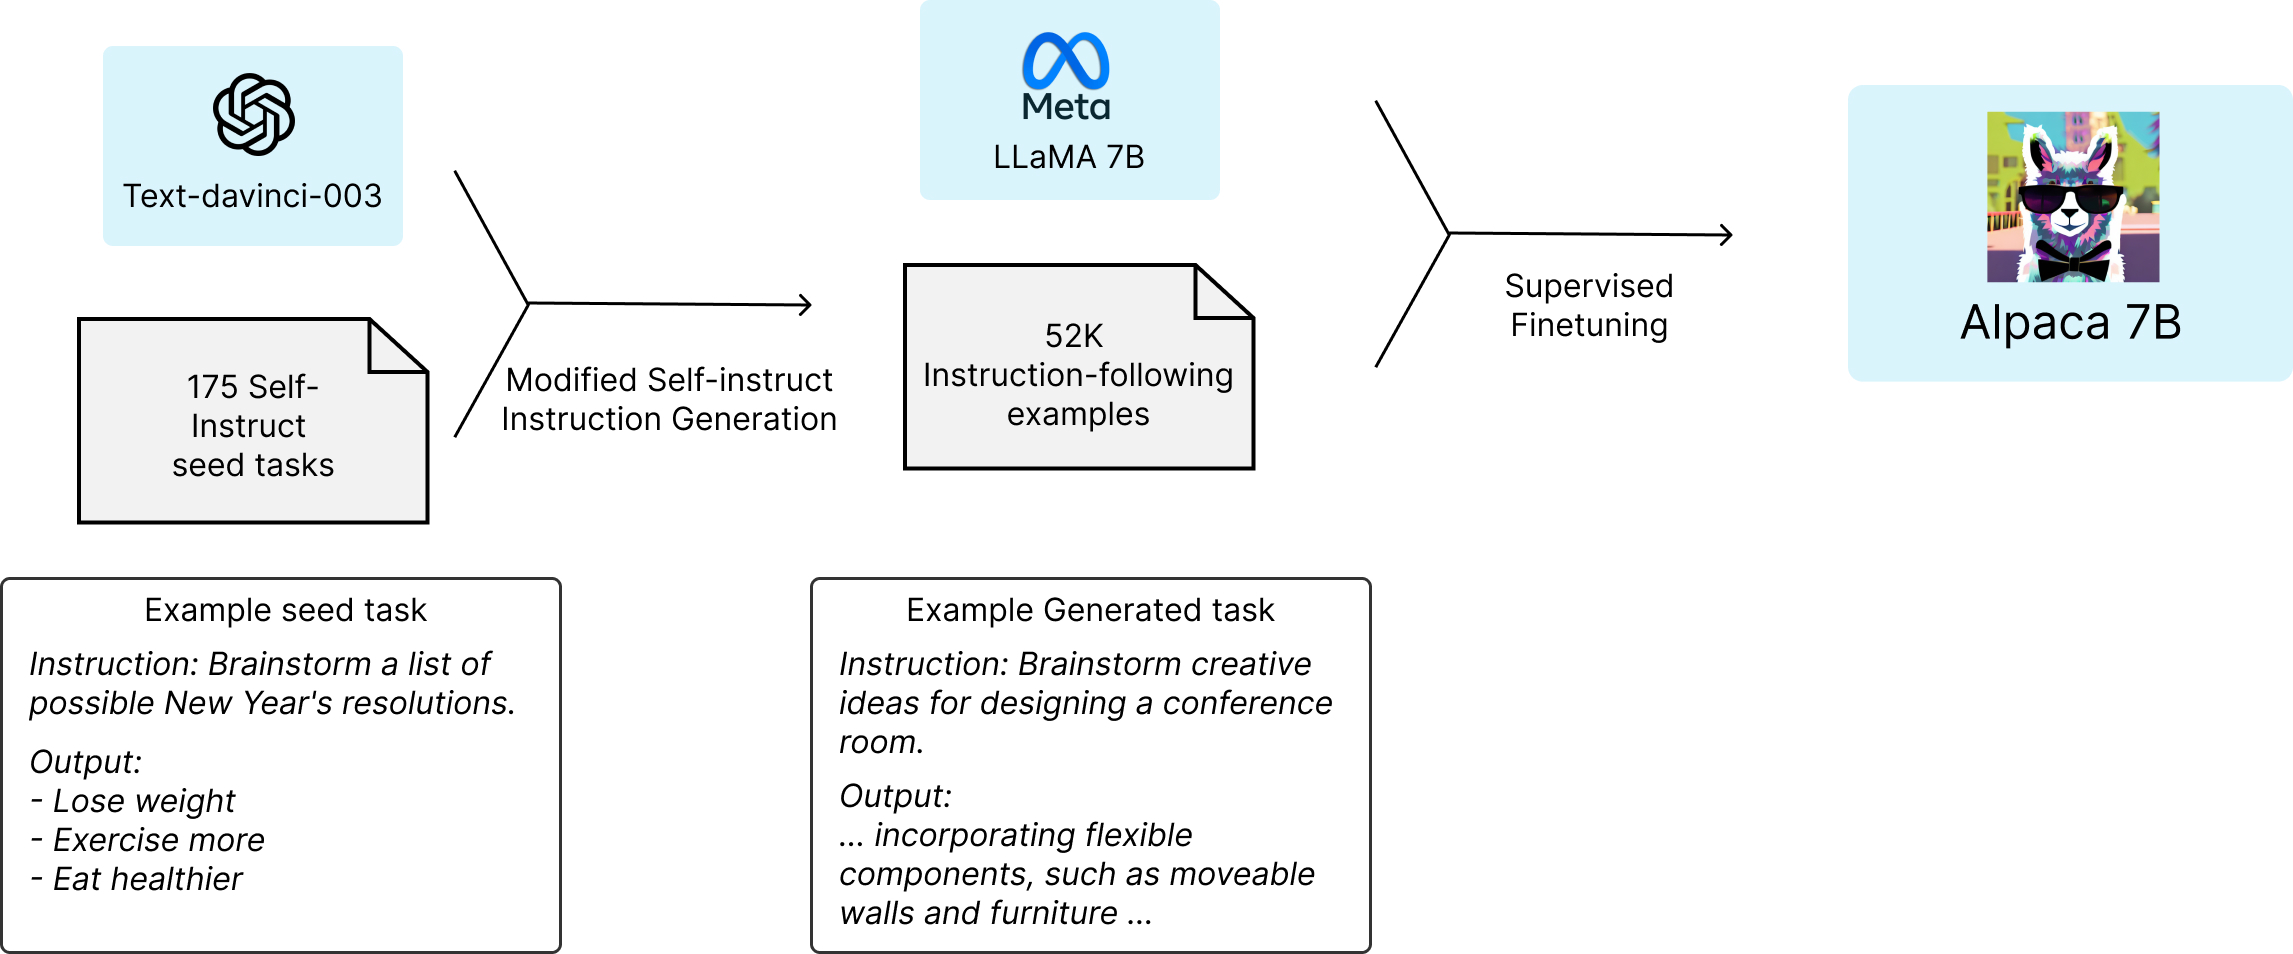
\includegraphics[width=17cm]{images/alpaca_framework.jpeg}}
        \caption[Overview of the Stanford Alpaca training procedure.]{Overview of the Stanford Alpaca training procedure.\\Figure by Taori et al. \cite{taoriStanfordCRFM}}
        \label{fig:alpaca_training}
    \end{figure}